Fermions are the quantized excitations of spinor fields and constitute all matter with spatial extent and conserved mass. They include the particles that form atoms, molecules, and macroscopic structures. Bosons, by contrast, act as force carriers: they mediate the interactions between fermions but do not constitute matter themselves. This division can be seen in the spin-based classification. Fermions possess half-integer spin ($\tfrac{1}{2}, \tfrac{3}{2}, \ldots$) and obey Fermi–Dirac statistics. Bosons have integer spin ($0, 1, 2, \ldots$) and obey Bose–Einstein statistics. This spin-based classification governs the symmetry of multi-particle wavefunctions and determines the existence or absence of exclusion principles. Fermions cannot share the same quantum state; bosons can.

The Standard Model includes four fundamental interactions. The electromagnetic force couples to electric charge and is mediated by the massless photon, a spin-1 boson. The weak force couples to weak isospin and hypercharge and is mediated by the $W^\pm$ and $Z^0$ bosons, which are massive spin-1 particles. The strong force acts on color charge and is mediated by eight massless spin-1 gluons, and described by the non-Abelian gauge group $\mathrm{SU}(3)$. The gravitational interaction is not described by the Standard Model but is expected to arise from a spin-2 field, with the hypothesized graviton as its mediator. All of these mediators are bosons. Only fermions — specifically quarks and leptons — carry the conserved quantum numbers associated with matter fields.

These force carriers differ fundamentally from fermions: they are not subject to exclusion and do not form matter in any persistent sense. Fermions, by contrast, are localized, quantized excitations of spinor fields, and every known material object is composed of them.

This group-theoretic distinction leads to a difference in statistical behavior. Fermions obey the Pauli exclusion principle: their total wavefunction is antisymmetric under particle exchange, preventing identical fermions from occupying the same quantum state. This antisymmetry governs atomic shell structure, the degeneracy pressure resisting gravitational collapse in white dwarfs and neutron stars, and the organization of electronic energy bands in solids. Bosons, in contrast, are symmetric under exchange and follow Bose–Einstein statistics, allowing them to occupy the same quantum state. This enables macroscopic quantum phenomena such as superfluidity, superconductivity, and stimulated emission in lasers. Fermions comprise what we call matter; bosons mediate the forces between them.

All known fermions fall into two fundamental families: quarks and leptons. Quarks carry color charge and couple to all four fundamental interactions: gravitational, electromagnetic, weak, and strong. Due to confinement, an emergent property of non-Abelian gauge symmetry in quantum chromodynamics, quarks cannot be isolated. Instead, they form composite bound states called hadrons. Baryons, such as protons and neutrons, consist of three quarks. Mesons, such as pions and kaons, are composed of a quark and an antiquark. These composites particles dominate the mass of ordinary matter.

Leptons, by contrast, do not carry color charge and are unaffected by the strong interaction. They are point-like to current experimental resolution, and couple via the weak force, gravity, and — if electrically charged — the electromagnetic force. The six known leptons are arranged into three generations, each containing one charged lepton and one corresponding neutrino:
\begin{itemize}
\item First generation: electron ($e^-$), electron neutrino ($\nu_e$)
\item Second generation: muon ($\mu^-$), muon neutrino ($\nu_\mu$)
\item Third generation: tau ($\tau^-$), tau neutrino ($\nu_\tau$)
\end{itemize}

The charged leptons differ in mass but are identical in spin and charge. The electron, with mass $0.511\,\text{MeV}/c^2$, is stable. The muon is 207 times more massive ($105.7\,\text{MeV}/c^2$) and decays with a mean lifetime of $2.2\,\mu$s. The tau lepton, at $1776.9\,\text{MeV}/c^2$, has a lifetime of $290$ femtoseconds. Neutrinos have no electric charge and interact only via the weak interaction and gravity. Their masses are known to be nonzero but extremely small — each less than $1\,\text{eV}/c^2$ — and remain difficult to measure directly.

Quarks mirror this generational hierarchy:
\begin{itemize}
\item First generation: up ($u$), down ($d$)
\item Second generation: charm ($c$), strange ($s$)
\item Third generation: top ($t$), bottom ($b$)
\end{itemize}
Each generation preserves the same electric charges and interaction types. The differences lie in mass and lifetime. Heavier quarks decay into lighter ones through weak interactions, conserving energy, momentum, and quantum numbers.

The existence of three fermion generations is an empirical fact, not a theoretical necessity. The Standard Model incorporates this structure through input parameters — masses, mixing angles, and decay constants — but offers no mechanism explaining the number of generations or the observed mass hierarchy. The replication appears arbitrary, though it affects all known particle behavior.

The muon exemplifies this. It is a second-generation charged lepton, with the same electric charge ($-1$), spin ($\tfrac{1}{2}$), and lepton number as the electron. Its decay proceeds through the weak interaction:
\[
\mu^- \rightarrow e^- + \bar{\nu}_e + \nu_\mu
\]
This three-body decay is mediated by virtual $W$ bosons and preserves lepton flavor. The muon's high mass and relatively long lifetime — among unstable particles — make it ideal for precision studies of lepton dynamics and relativistic motion.

Muons are produced copiously in Earth’s upper atmosphere. The initiating agents are primary cosmic rays, consisting mostly of high-energy protons with energies from a few GeV up to $10^{20}$ eV. These protons collide with atmospheric nuclei at altitudes of 10–20 km, producing hadronic showers that include pions and kaons. The relevant decay modes are:
\[
\pi^+ \rightarrow \mu^+ + \nu_\mu, \qquad \pi^- \rightarrow \mu^- + \bar{\nu}_\mu
\]
Pions decay with a lifetime of $26\,\text{ns}$ in their rest frame. Because they are often highly relativistic, their decay products inherit both energy and directionality. Muons generated this way arrive at Earth’s surface with typical energies of 1–10 GeV and velocities exceeding $0.995c$.

A muon at rest lives $2.2\,\mu$s. At relativistic speed, this would classically limit its travel distance to:
\[
d_{\text{classical}} = v \cdot \tau_0 \approx 3 \times 10^8\,\text{m/s} \cdot 2.2 \times 10^{-6}\,\text{s} \approx 660\,\text{m}
\]
Yet detectors regularly observe muons at sea level and below, sometimes even in deep underground laboratories. The classical estimate underpredicts by more than an order of magnitude.

The explanation is time dilation. From the Earth frame, the muon's proper lifetime is extended by the Lorentz factor:
\[
\tau = \gamma \tau_0, \qquad \gamma = \frac{1}{\sqrt{1 - v^2/c^2}}
\]
For $v \approx 0.998c$, $\gamma \approx 15$, implying an effective lifetime of about $33\,\mu$s. This allows the muon to traverse approximately 10 kilometers before decaying — consistent with both experimental detection rates and relativistic kinematics.

From the muon’s rest frame, the explanation is spatial contraction. The Earth’s atmosphere is contracted along the direction of motion by the same factor $\gamma$. A journey from 15 km altitude contracts to 1 km in the muon’s frame, easily traversable within its rest-frame lifetime. Both frames yield consistent predictions — this symmetry illustrates the covariance of physical laws under Lorentz transformations.

Muon detection exploits their charge, mass, and penetrating power. Being electrically charged, muons ionize matter as they pass through. Scintillation counters, Cherenkov detectors, drift chambers, and resistive plate chambers are common technologies for tracking these particles. The most basic detection scheme involves a scintillator material coupled to a photomultiplier tube: when a muon passes through the scintillator, it excites molecules which re-emit photons, triggering a measurable pulse of light. In cloud chambers and bubble chambers, the muon leaves a visible track by ionizing a supersaturated or superheated medium. More advanced systems use layered arrangements of materials and timing electronics to reconstruct particle trajectories and momenta.

Muon energy loss in matter is relatively small, owing to their mass — 207 times that of the electron — which suppresses bremsstrahlung, pair production, and photonuclear interactions. As a result, muons can pass through several meters of rock or dense material with only modest energy attenuation. At sea level, the vertical muon flux is approximately one per square centimeter per minute. This makes them the dominant component of secondary cosmic radiation at Earth’s surface, and they play a significant role in radiography, background calibration in neutrino detectors, and long-baseline experiments in particle physics.

The observation of atmospheric muons provided one of the earliest natural confirmations of relativistic time dilation. Unlike laboratory-bound tests requiring synchronized atomic clocks or controlled accelerators, muon flux at sea level confirms relativistic predictions using naturally occurring particles and passive detection methods. The agreement between laboratory decay rates and atmospheric propagation distances offers direct evidence that relativistic time transformation is a physical reality, not merely a mathematical artifact.

\newpage
\thispagestyle{empty}
\begin{center}
\vspace*{2em}
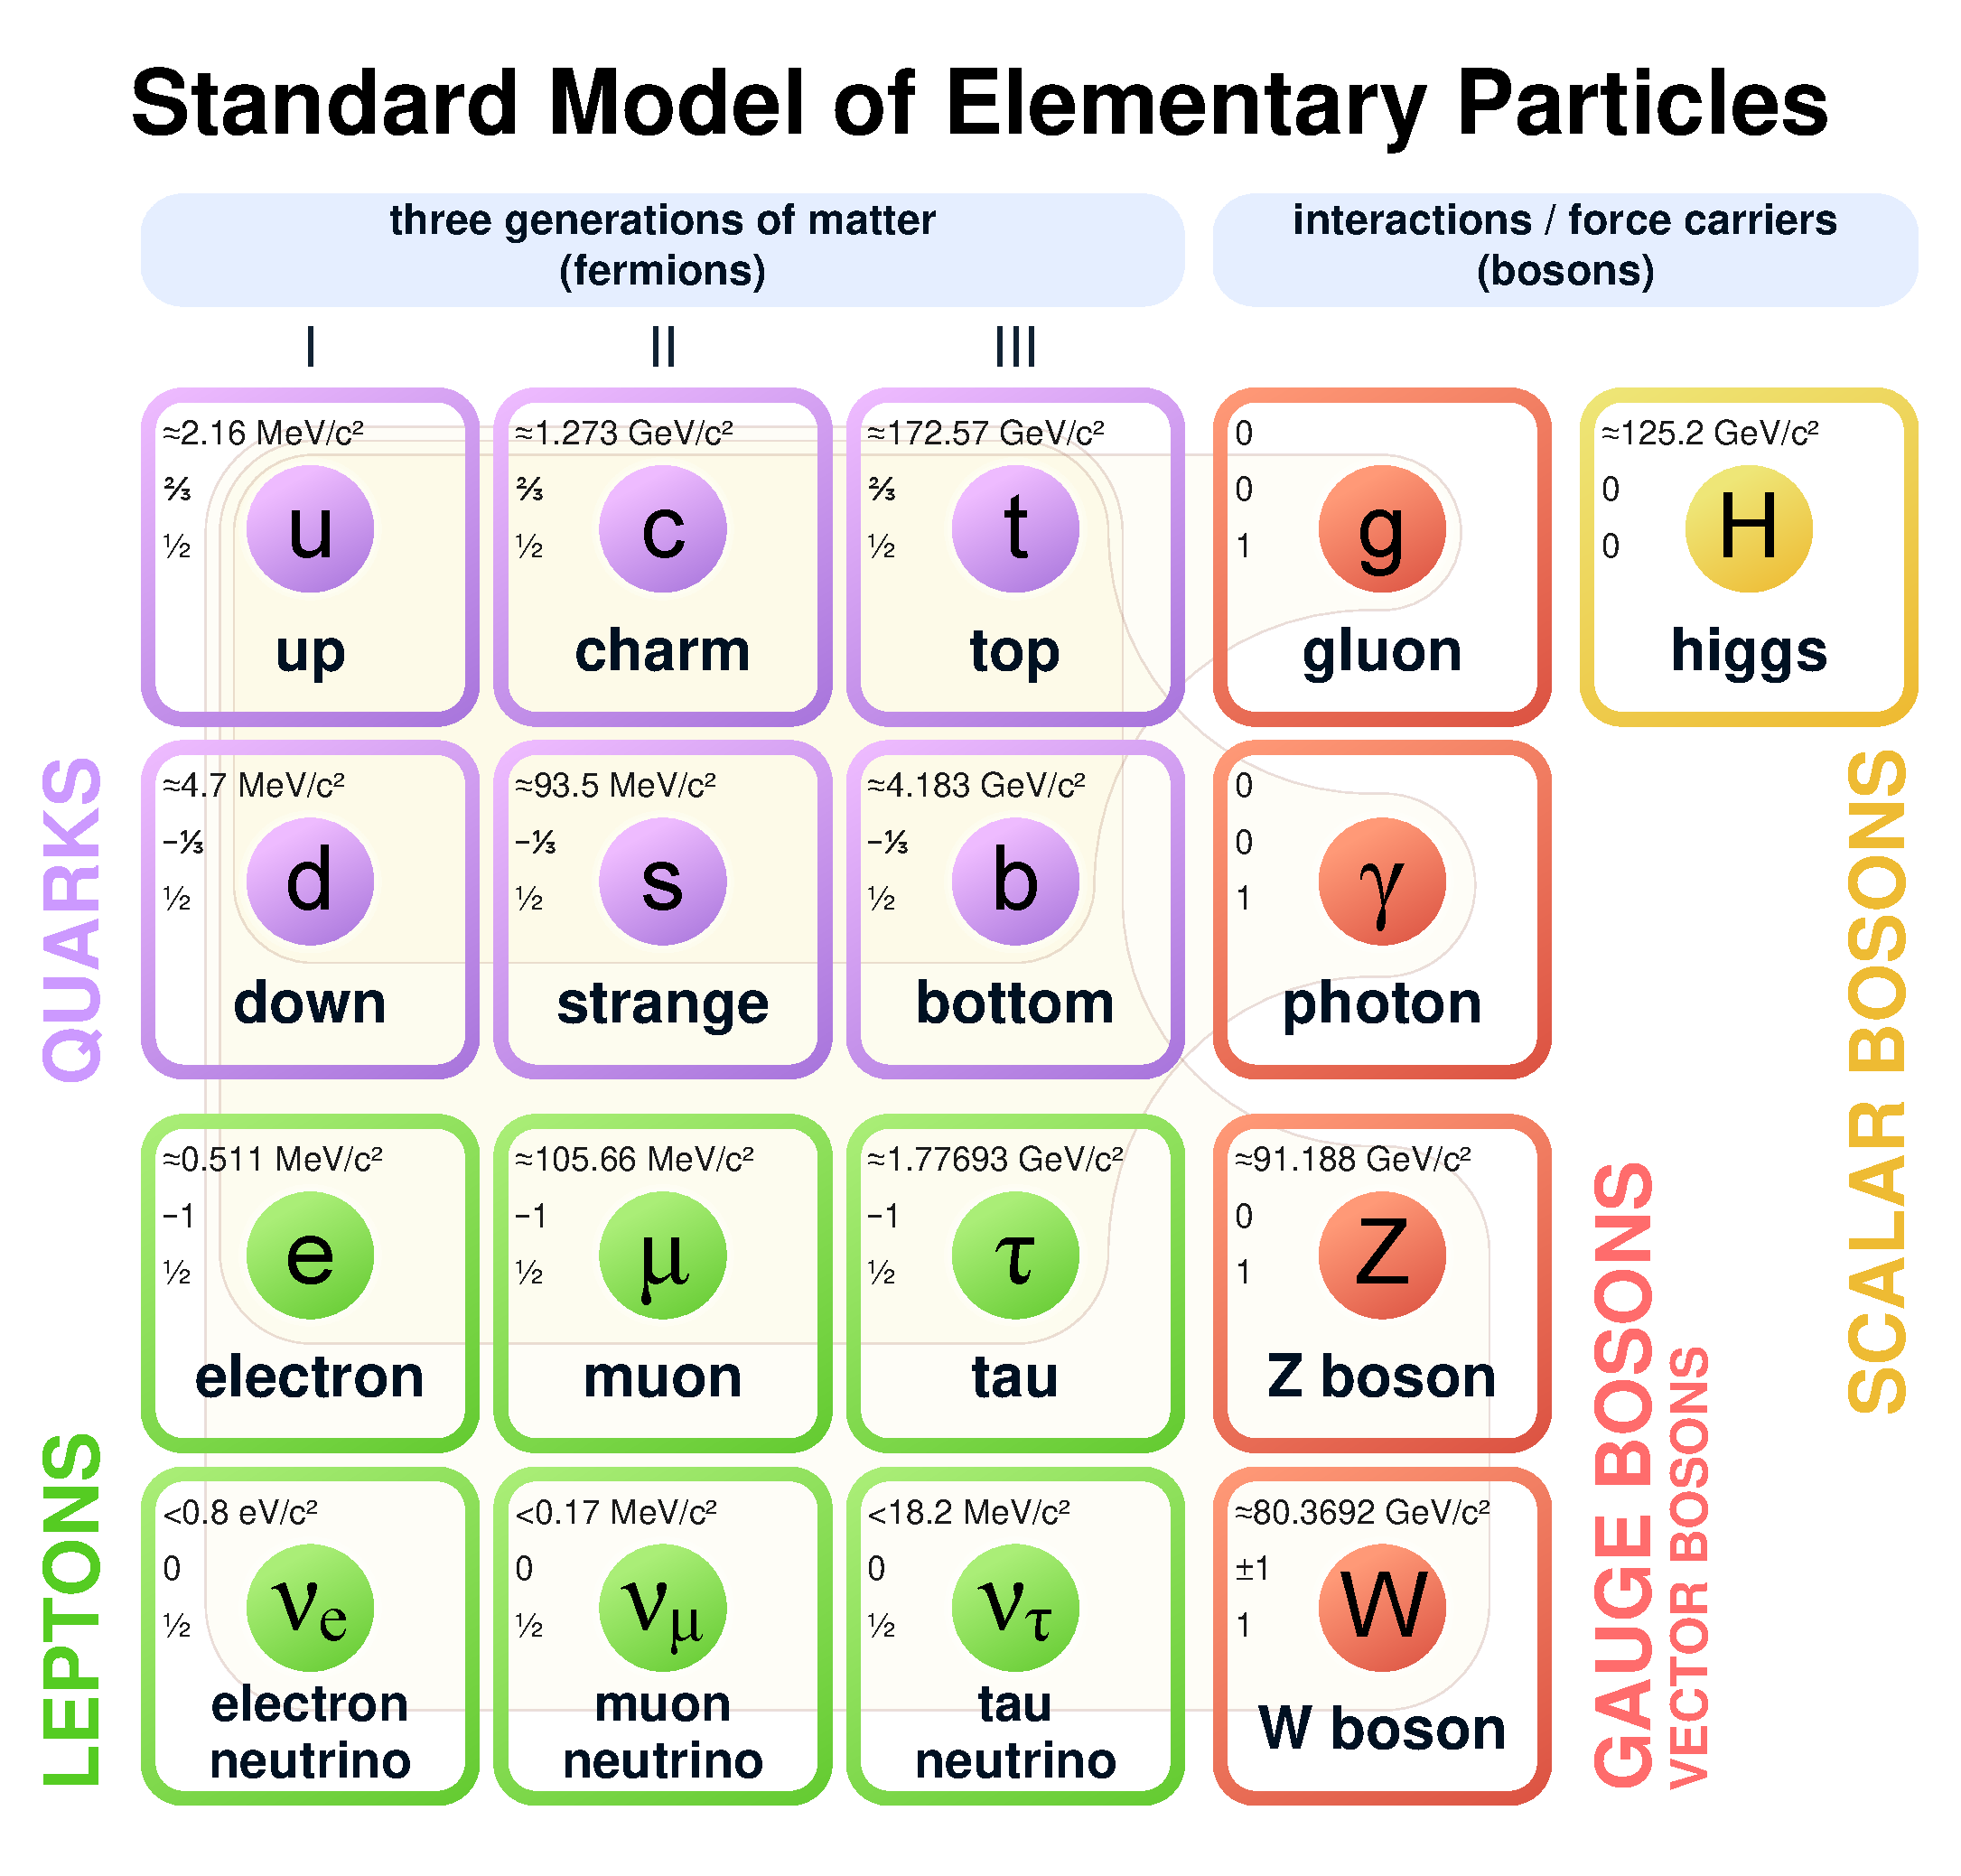
\includegraphics[width=0.8\textwidth]{19_CosmicRayMuons/Standard_Model_of_Elementary_Particles.pdf}
\vspace{2em}
\end{center}